\section{Time Class Reference}
\label{classTime}\index{Time@{Time}}
Inheritance diagram for Time::\begin{figure}[H]
\begin{center}
\leavevmode
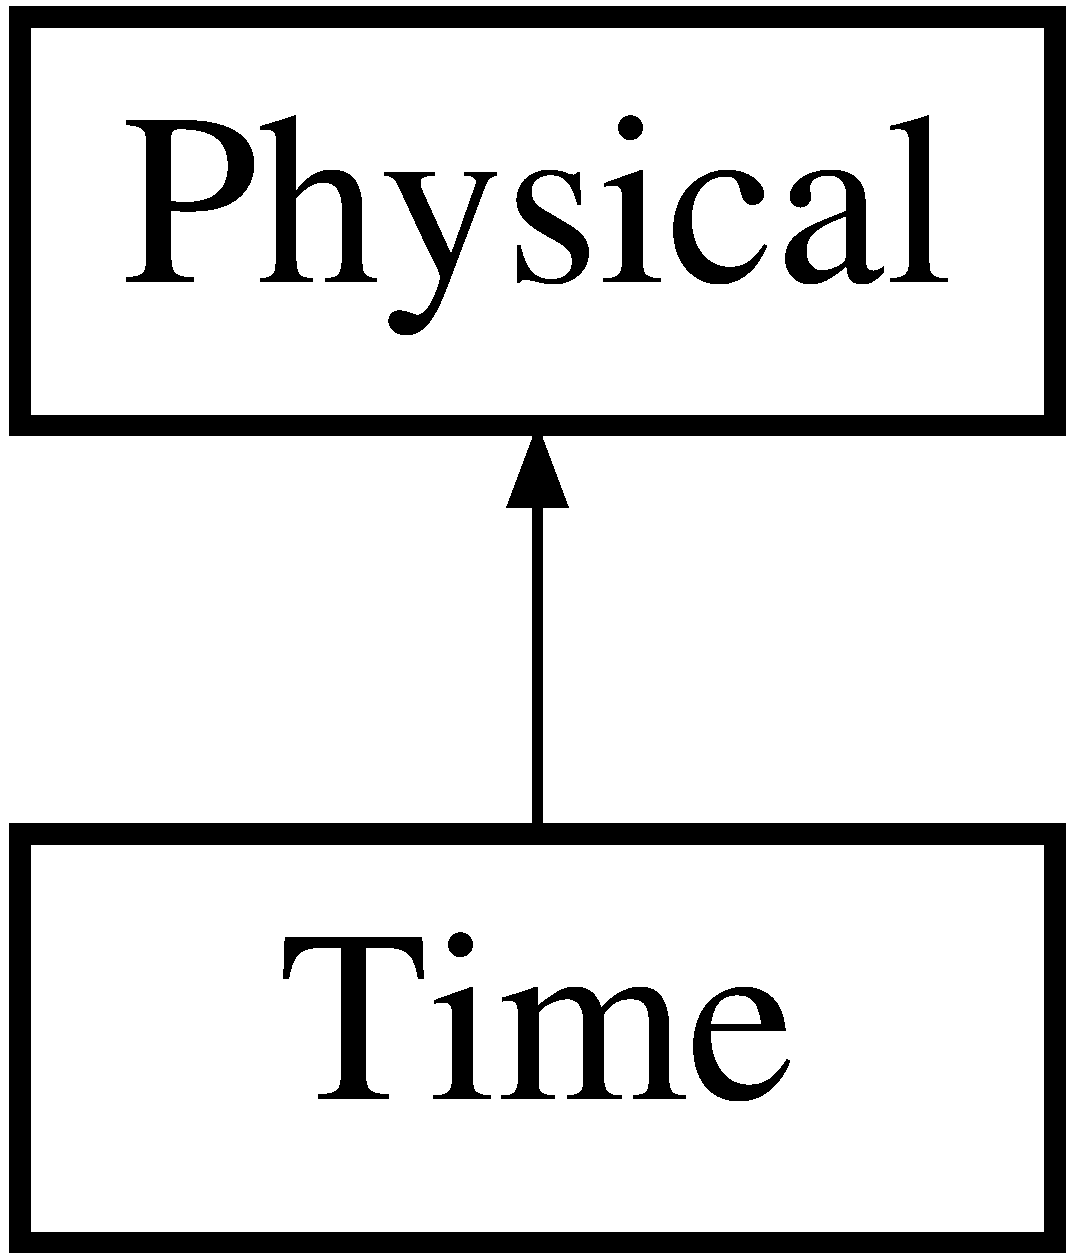
\includegraphics[height=2cm]{classTime}
\end{center}
\end{figure}


\subsection{Detailed Description}
The time. 

This class is responsable for governing the simulation progress. \subsection*{Public Member Functions}
\begin{CompactItemize}
\item 
{\bf Time} (double timestep)\label{classTime_99767f8eeafc75912229851f484ac55a}

\begin{CompactList}\small\item\em Create time. \item\end{CompactList}\item 
virtual {\bf $\sim$Time} ()\label{classTime_daddb2dc46aa0b725cafe2e6cc8b8a5a}

\begin{CompactList}\small\item\em Destroy time. \item\end{CompactList}\item 
virtual string {\bf getPhysicalDescription} ()\label{classTime_1ac1a866153ab2dd80abf20b6e923909}

\begin{CompactList}\small\item\em Return physick description. \item\end{CompactList}\item 
void {\bf run} (unsigned long long steps, ostream \&log=cout)
\begin{CompactList}\small\item\em Run simulation for all attached objects. \item\end{CompactList}\item 
void {\bf run} (unsigned long long events, class {\bf StochasticEventGenerator} $\ast$eventSource, unsigned long long maxSteps, ostream \&log=cout)
\begin{CompactList}\small\item\em Run simulation for all attached objects. \item\end{CompactList}\item 
void {\bf runNested} (unsigned long long steps, unsigned long long runs, {\bf DataCollector} $\ast$runRecorder, ostream \&log=cout)
\begin{CompactList}\small\item\em Run multiple simulations for all attached objects. \item\end{CompactList}\item 
void {\bf runNested} (unsigned long long events, class {\bf StochasticEventGenerator} $\ast$eventSource, unsigned long long maxSteps, unsigned long long runs, {\bf DataCollector} $\ast$runRecorder, ostream \&log=cout)
\begin{CompactList}\small\item\em Run multiple simulations for all attached objects. \item\end{CompactList}\item 
void {\bf add} (class {\bf TimeDependent} $\ast$object)\label{classTime_024e5e623073cb5e57f3d372aa73ac8e}

\begin{CompactList}\small\item\em Attach an object. \item\end{CompactList}\item 
void {\bf add} (class {\bf Estimator} $\ast$object)\label{classTime_7f708047aa102b67e62612decf90441c}

\begin{CompactList}\small\item\em Attach an object. \item\end{CompactList}\item 
void {\bf remove} (class {\bf TimeDependent} $\ast$object)\label{classTime_8c0290a43c118078cfdd824e57ac6723}

\begin{CompactList}\small\item\em Detach an object. \item\end{CompactList}\item 
void {\bf remove} (class {\bf Estimator} $\ast$object)\label{classTime_12019d8f5cc8a47d50cd1ac8e77ee4ca}

\begin{CompactList}\small\item\em Detach an object. \item\end{CompactList}\end{CompactItemize}


\subsection{Member Function Documentation}
\index{Time@{Time}!run@{run}}
\index{run@{run}!Time@{Time}}
\subsubsection[run]{\setlength{\rightskip}{0pt plus 5cm}void Time::run (unsigned long long {\em steps}, \/  ostream \& {\em log} = {\tt cout})}\label{classTime_0a03cab1c544cfac3fb164d39651710d}


Run simulation for all attached objects. 

Runs a simulation for a certain number of time steps. \begin{Desc}
\item[Parameters: ]\par
\begin{description}
\item[{\em 
steps}]number of time steps to run \item[{\em 
log}]stream for progress messages \end{description}
\end{Desc}
\index{Time@{Time}!run@{run}}
\index{run@{run}!Time@{Time}}
\subsubsection[run]{\setlength{\rightskip}{0pt plus 5cm}void Time::run (unsigned long long {\em events}, \/  class {\bf StochasticEventGenerator} $\ast$ {\em eventSource}, \/  unsigned long long {\em maxSteps}, \/  ostream \& {\em log} = {\tt cout})}\label{classTime_1918f0b5253217405077d487838f8e16}


Run simulation for all attached objects. 

Runs a simulation for a certain number of events (e.g. spikes from a neuron). As a safeguard a maximum number of time steps must be given, in case the event source fails to deliver events. \begin{Desc}
\item[Parameters: ]\par
\begin{description}
\item[{\em 
events}]number of events until run is finished \item[{\em 
eventSource}]event source \item[{\em 
maxSteps}]maximum number of time steps, should the event source fail \item[{\em 
log}]stream for progress messages \end{description}
\end{Desc}
\index{Time@{Time}!runNested@{runNested}}
\index{runNested@{runNested}!Time@{Time}}
\subsubsection[runNested]{\setlength{\rightskip}{0pt plus 5cm}void Time::runNested (unsigned long long {\em steps}, \/  unsigned long long {\em runs}, \/  {\bf DataCollector} $\ast$ {\em runRecorder}, \/  ostream \& {\em log} = {\tt cout})}\label{classTime_60e45b336cd984cf682d5c4b760cfcf7}


Run multiple simulations for all attached objects. 

Runs a number of simulations for a certain number of time steps. \begin{Desc}
\item[Parameters: ]\par
\begin{description}
\item[{\em 
steps}]number of time stepsfor each run \item[{\em 
runs}]number of time runs \item[{\em 
runRecorder}]object with functions to execute at beginning/end of each run \item[{\em 
log}]stream for progress messages \end{description}
\end{Desc}
\index{Time@{Time}!runNested@{runNested}}
\index{runNested@{runNested}!Time@{Time}}
\subsubsection[runNested]{\setlength{\rightskip}{0pt plus 5cm}void Time::runNested (unsigned long long {\em events}, \/  class {\bf StochasticEventGenerator} $\ast$ {\em eventSource}, \/  unsigned long long {\em maxSteps}, \/  unsigned long long {\em runs}, \/  {\bf DataCollector} $\ast$ {\em runRecorder}, \/  ostream \& {\em log} = {\tt cout})}\label{classTime_3f2d3b41a6bc9d8b1cea4de58fdf3674}


Run multiple simulations for all attached objects. 

Runs a number of simulations for a certain number of time steps. \begin{Desc}
\item[Parameters: ]\par
\begin{description}
\item[{\em 
events}]number of events until run is finished \item[{\em 
eventSource}]event source \item[{\em 
maxSteps}]maximum number of time steps, should the event source fail \item[{\em 
runs}]number of time runs \item[{\em 
runRecorder}]object with functions to execute at beginning/end of each run \item[{\em 
log}]stream for progress messages \end{description}
\end{Desc}
